\documentclass[a4paper,12pt,final]{article}

\usepackage[margin=1in]{geometry}
\usepackage{graphicx}
\title{
\begin{center}
  	
\includegraphics[scale=0.3]{101Logo.png} 
  \end{center}
  \textbf{\\}
CSIR - Distributed Application Manager\\
Functional Requirements and Design Document\\
}
\author{101 Solutions}

\begin{document}
\maketitle
\begin{center}
Version 1.3
\end{center}
\textbf{\\}
\textbf{\\}
\textbf{\\}
\textbf{\\}
\textbf{\\}
\textbf{\\}
\begin{center}
\begin{tabular}{|l|l|}
\hline
Francois Germishuizen & 11093618\\
\hline
Jaco Swanepoel & 11016354\\
\hline
Henko van Koesveld & 11009315\\
\hline
\end{tabular}
\end{center}
\thispagestyle{empty}
\newpage
\thispagestyle{empty}
\textbf{\large{Change Log}}
\vspace{6pt}\newline
\begin{tabular}{|l|l|l|l|}
\hline
\textbf{Date} & \textbf{Version} & \textbf{Description} & \textbf{Done by}\\
\hline
13 Sept & Version 0.1 & Document Created & Jaco\\
\hline
13 Sept & Version 0.2 & Added usecase diagrams & Jaco\\
\hline
13 Sept & Version 0.3 & Added AddBuild, RequestSysInfo and  & Jaco\\
&&GetSysInfo usecase&\\
\hline
13 Sept & Version 0.4 & Added Upcoming usecases and Simulations & Jaco\\
\hline
13 Sept & Version 0.5 & Added overall processes and adjusted margins & Jaco\\
\hline
13 Sept & Version 0.6 & Added AddSlave, StartServer, StopServer  & Jaco\\
&&and SetPort usecase&\\
\hline
13 Sept & Version 0.7 & Added Glossary & Jaco\\
\hline
13 Sept & Version 0.8 & Added Class diagrams & Jaco\\
\hline
13 Sept & Version 0.9 & Added AddBuild via network usecase & Jaco\\
\hline
13 Sept & Version 1.0 & Added description of communication diagrams & Henko\\
\hline
15 Sept & Version 1.1 & Final grammar check & Jaco\\
\hline
10 Oct & Version 1.2 & Added simulations to Use cases away from upcoming & Jaco\\
\hline
12 Oct & Version 1.3 & Updated usecase diagrams & Jaco\\
\hline
\end{tabular}
\newpage
\tableofcontents
\thispagestyle{empty}
\newpage

\pagenumbering{arabic}
\section{Overview}
\subsection{Background}
The CSIR is actively developing a distributed simulation framework that ties
in with various other real systems and is used to exchange information
between them. The client has a number of configurations of this system
depending on the requirements of the client which can involve various
external applications as well.\\
\textbf{\\}
One of the issues the client has is to quickly distribute the latest build or
configuration files of their software over various computers that are needed
for an experiment. In some cases the same computers may be used for other
experiments which mean each of the computers may need to have various
builds and configuration options.\\
\textbf{\\}
Another issue they experience is the running, stopping and restarting of
the complete simulation. During a simulation it may be determined that
certain configuration options may need to be changed and distributed to the
affected machines, in which case either all or some components will need to
be restarted which can become tedious and time consuming.
\subsection{Business opportunity}
The goal of our project is to develop an application which is able to maintain
various build versions of the simulation framework and distribute these builds
to certain designated machines that may be required for an experiment. The
application will monitor system statistics of the various machines attached
to an experiment and will have the ability to execute applications on those
machines which will have different configuration options.\\
\textbf{\\}
The application will consist of a master and slave component where the
master is used to control the distribution of slaves. From the master one will
be able to start an experiment which will run the relevant applications on all
the necessary machines.




\newpage
\section{Use Cases}
We have both a master and slave application. The master is called AppMan and the slave is called AppManClient.\\
\textbf{\\}
Below is a use case of the AppMan system as it currently is:\\
\begin{center}
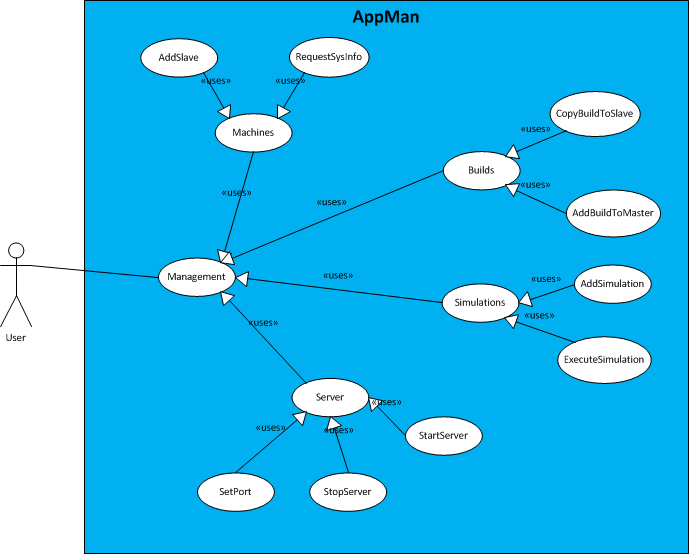
\includegraphics[scale=0.8]{AppManUseCase.png}
\end{center}
Below is a use case diagram of the AppManClient system as it currently is:\\
\begin{center}
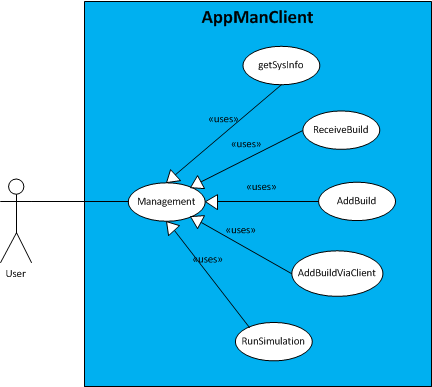
\includegraphics[scale=0.7]{AppManClientUseCase.png}
\end{center}


\subsection{AddBuild usecase}
The following activity diagram is applicable to both AddBuildToMaster in AppMan as well as AddBuildViaClient in AppManClient.\\
\textbf{\\}
\begin{center}
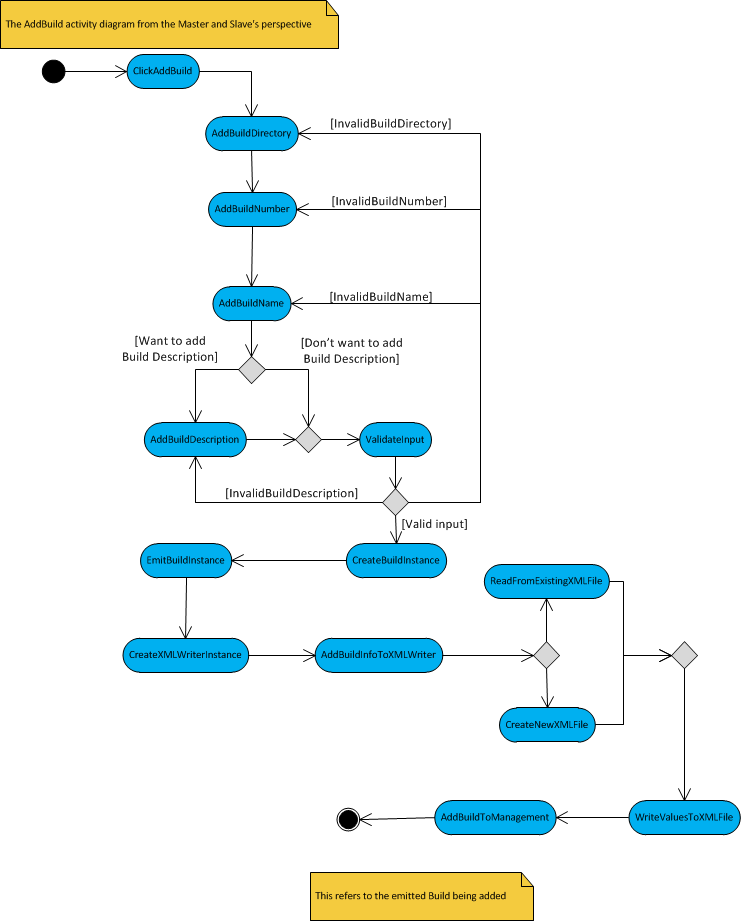
\includegraphics[scale=0.8]{AddBuildActivity.png}
\end{center}


\subsection{RequestSysInfo usecase}
The following activity diagram is applicable to the RequestSysInfo usecase in AppMan.\\
\textbf{\\}
\begin{center}
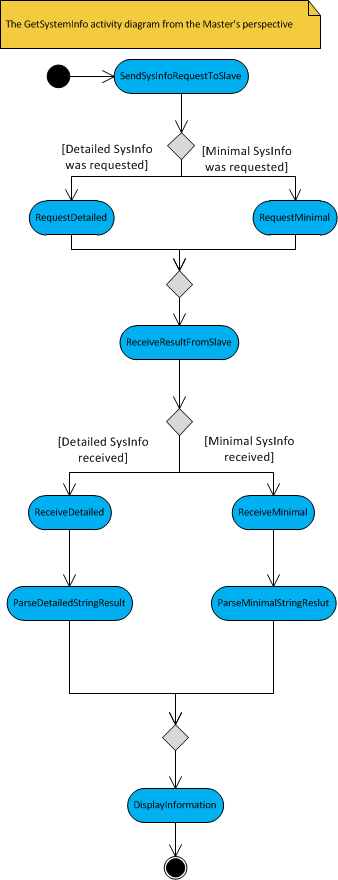
\includegraphics[scale=0.95]{GetSystemInfoActivityMASTER.png}
\end{center}


\subsection{GetSysInfo usecase}
The following activity diagram is applicable to the GetSysInfo usecase in AppManClient.\\
\textbf{\\}
\begin{center}
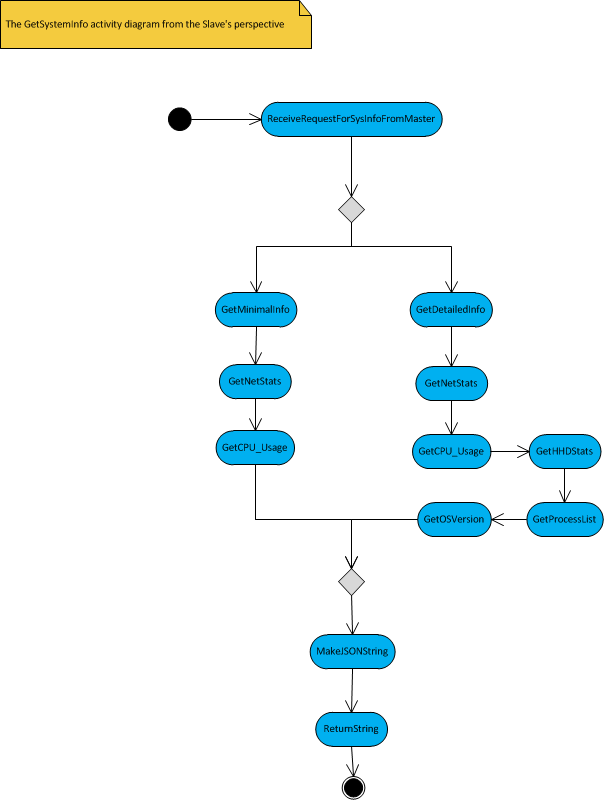
\includegraphics[scale=1]{GetSystemInfoActivitySLAVE.png}
\end{center}




\subsection{AddSlave usecase}
The following activity diagram is applicable to the AddSlave usecase in AppMan.\\
\textbf{\\}
\begin{center}
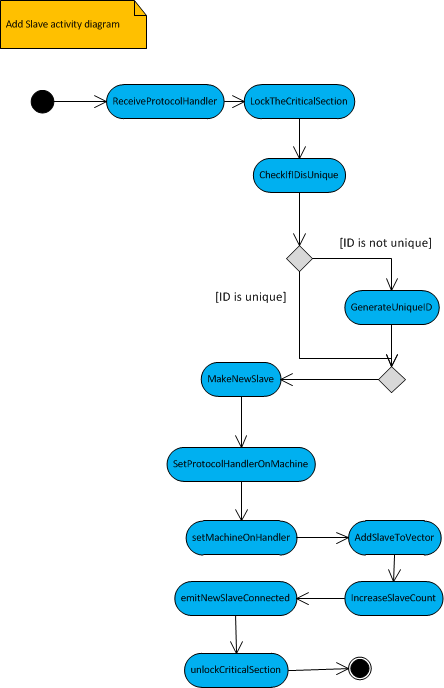
\includegraphics[scale=1]{AddSlaveActivity.png}
\end{center}



\newpage
\subsection{AddBuild via network usecase}
The following activity diagram is applicable to the AddBuild usecase in AppManClient.\\
\textbf{\\}
\begin{center}
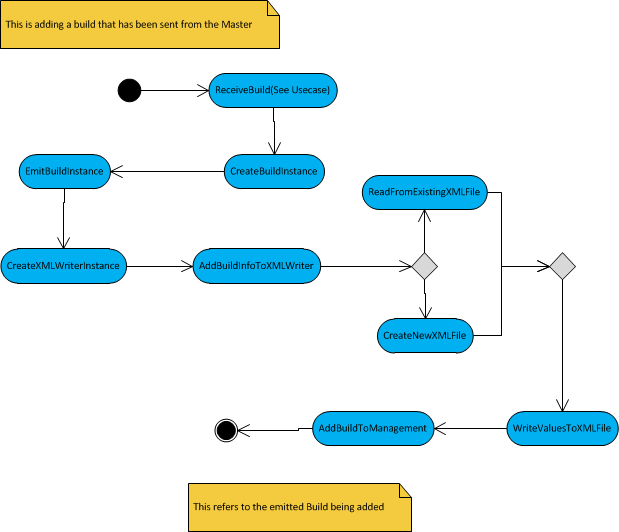
\includegraphics[scale=1]{AddBuildSlaveActivity.png}
\end{center}



\newpage
\subsection{StartServer usecase}
The following activity diagram is applicable to the StartServer usecase in AppMan.\\
\textbf{\\}
\begin{center}
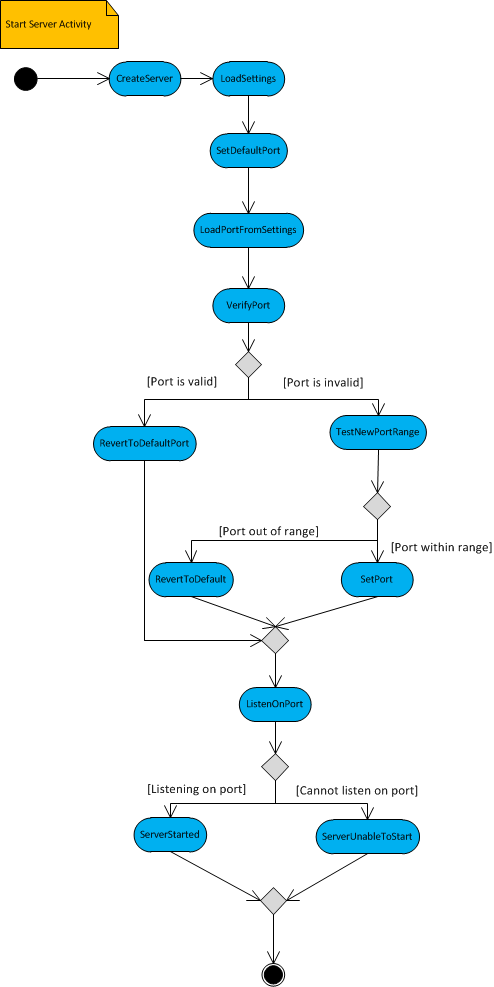
\includegraphics[scale=0.8]{StartServer.png}
\end{center}




\newpage
\subsection{SetPort usecase}
The following activity diagram is applicable to the SetPort usecase in AppMan.\\
\textbf{\\}
\begin{center}
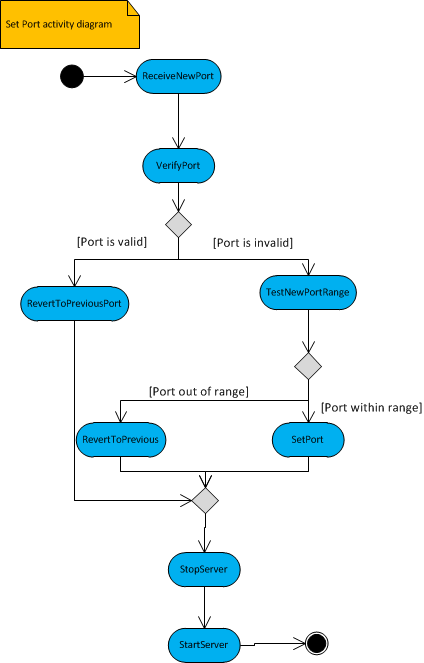
\includegraphics[scale=1]{SetPort.png}
\end{center}




\newpage
\subsection{StopServer usecase}
The following activity diagram is applicable to the StopServer usecase in AppMan.\\
\textbf{\\}
\begin{center}
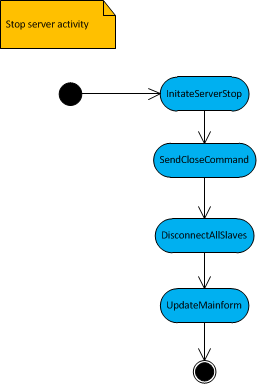
\includegraphics[scale=1]{StopServer.png}
\end{center}

\newpage

\subsection{AddSimulation}
A simulation must be added to AppMan in the following way:
\begin{center}

\includegraphics[scale=0.9]{AddSimulationActivity.png}
\end{center}

\newpage
\subsection{RunSimulation AppMan}
A simulation is run from AppMan in the following way:
\begin{center}
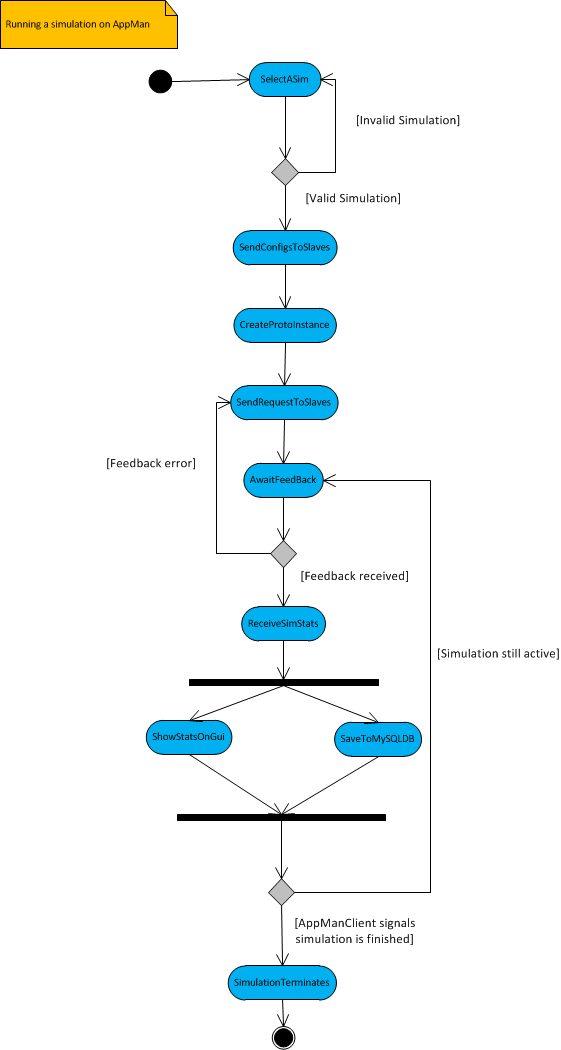
\includegraphics[scale=0.8]{RunningASimOnAppMan.png}
\end{center}

\newpage
\subsection{RunSimulation AppManClient}
A simulation is run from AppManClient in the following way:
\begin{center}
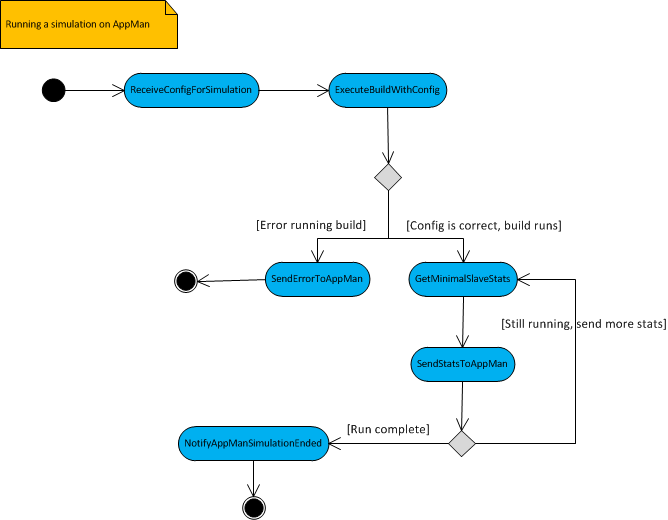
\includegraphics[scale=0.9]{RunningASimOnAppManClient.png}
\end{center}








\newpage
\section{Class diagrams}
\subsection{AppMan Class Diagram}
Due to its large size, the class diagram is split into multiple, seperate diagrams. Classes will be repeated to show how they all link.\\
\begin{center}
	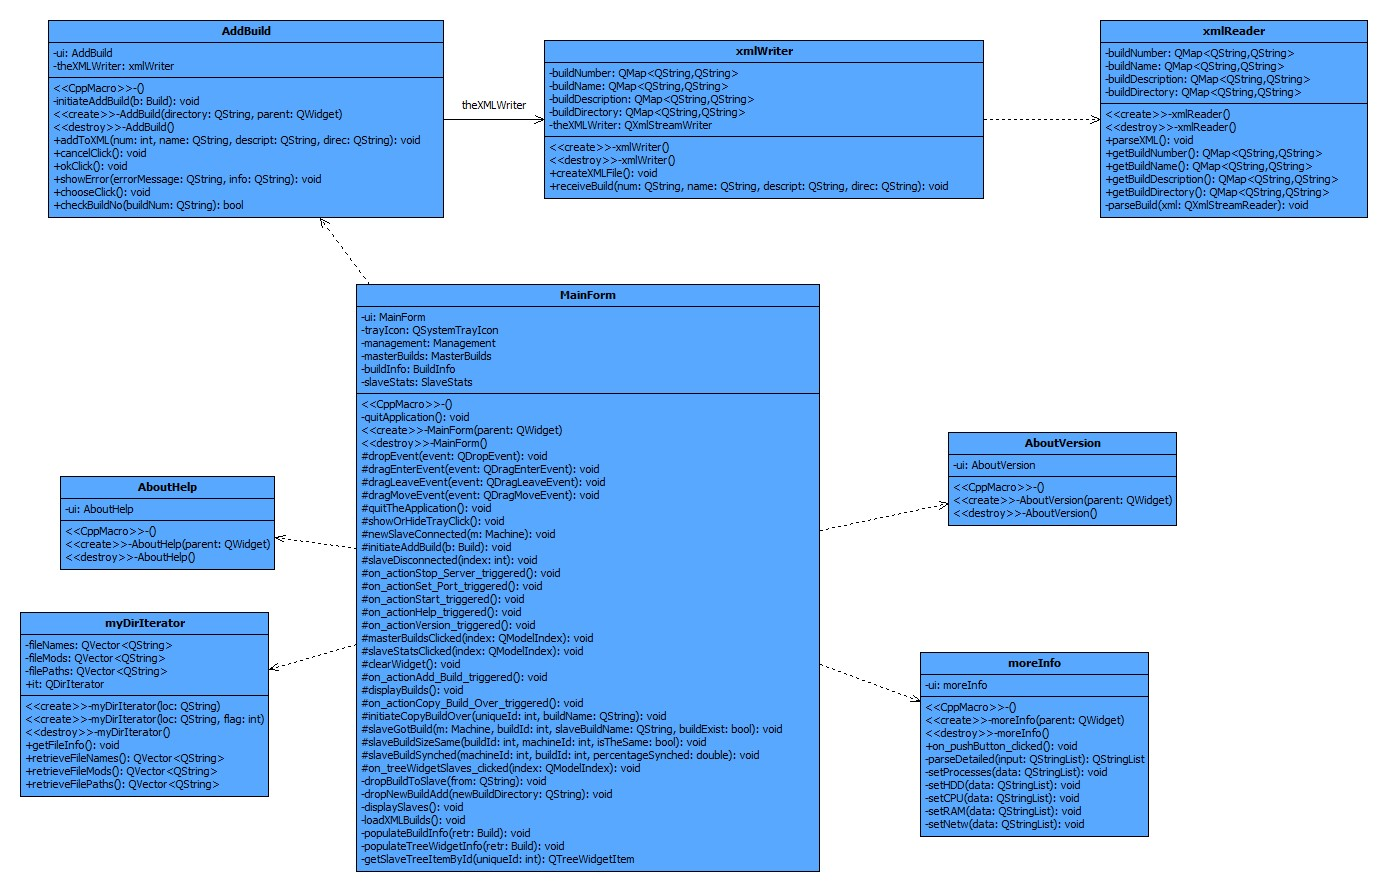
\includegraphics[angle = 90,scale = 0.42]{MainformNew.jpg}
\end{center}
\begin{center}
	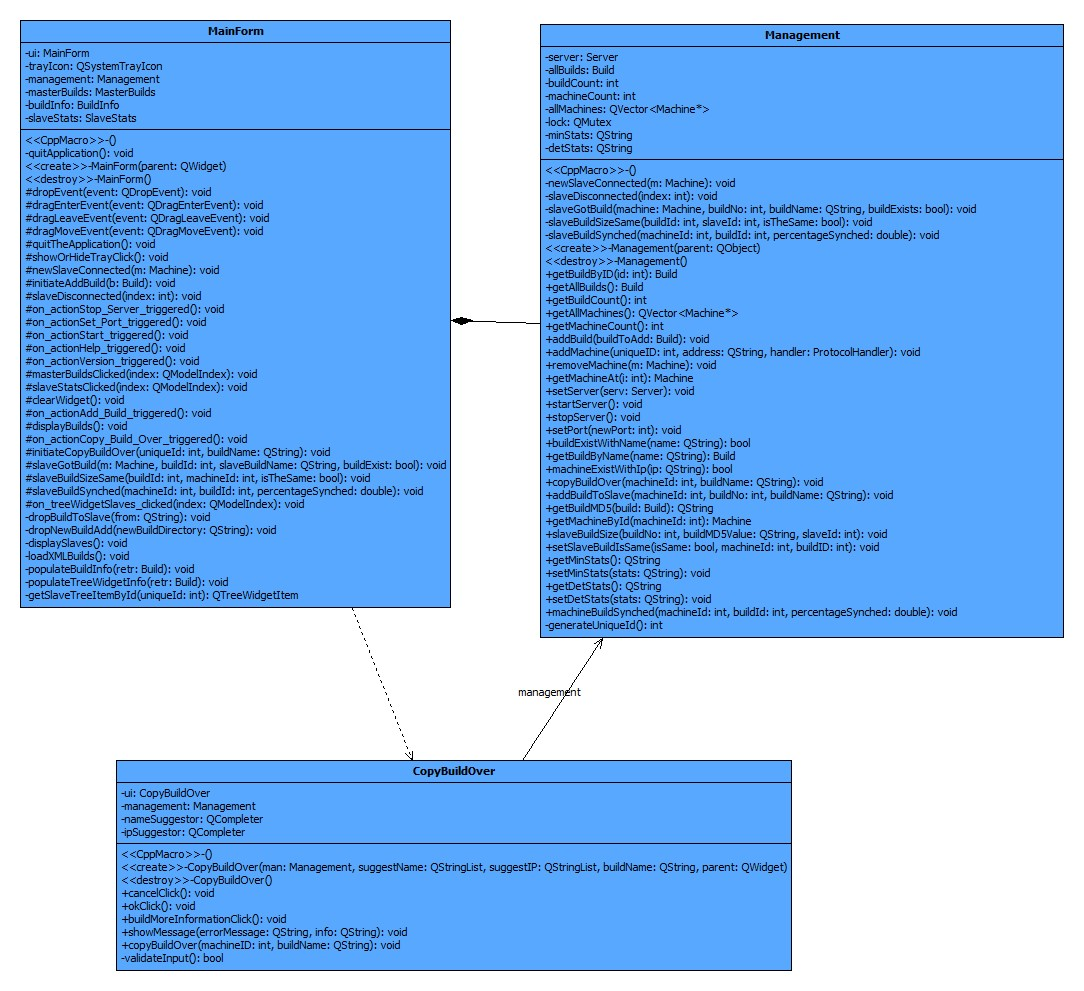
\includegraphics[angle = 90,scale = 0.5]{Mainformnew2.jpg}
\end{center}
\begin{center}
	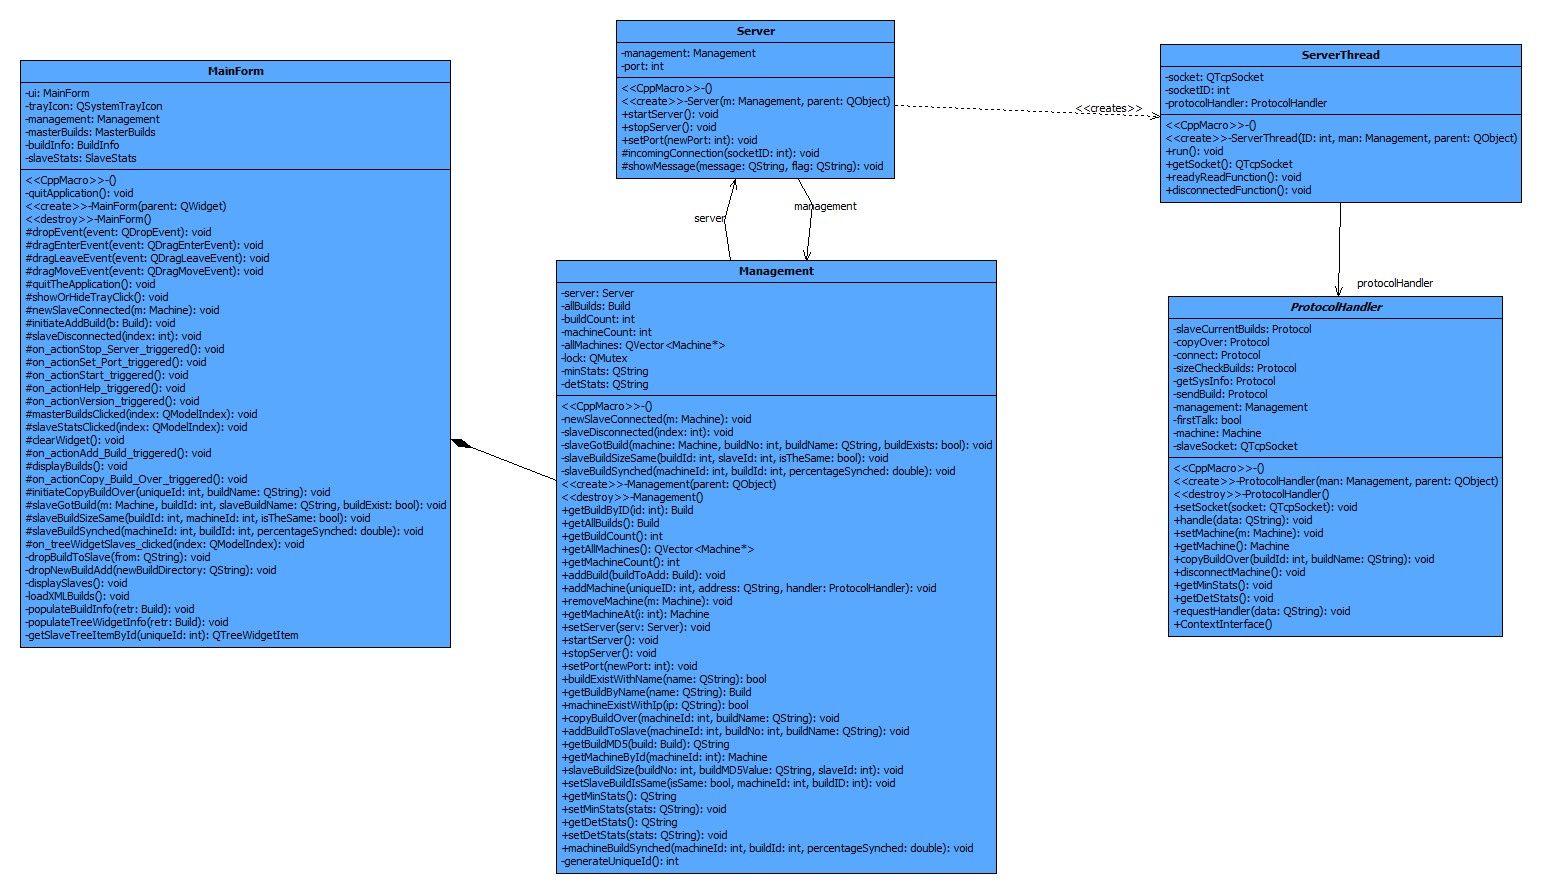
\includegraphics[angle = 90,scale = 0.45]{Server.jpg}
\end{center}
\begin{center}
	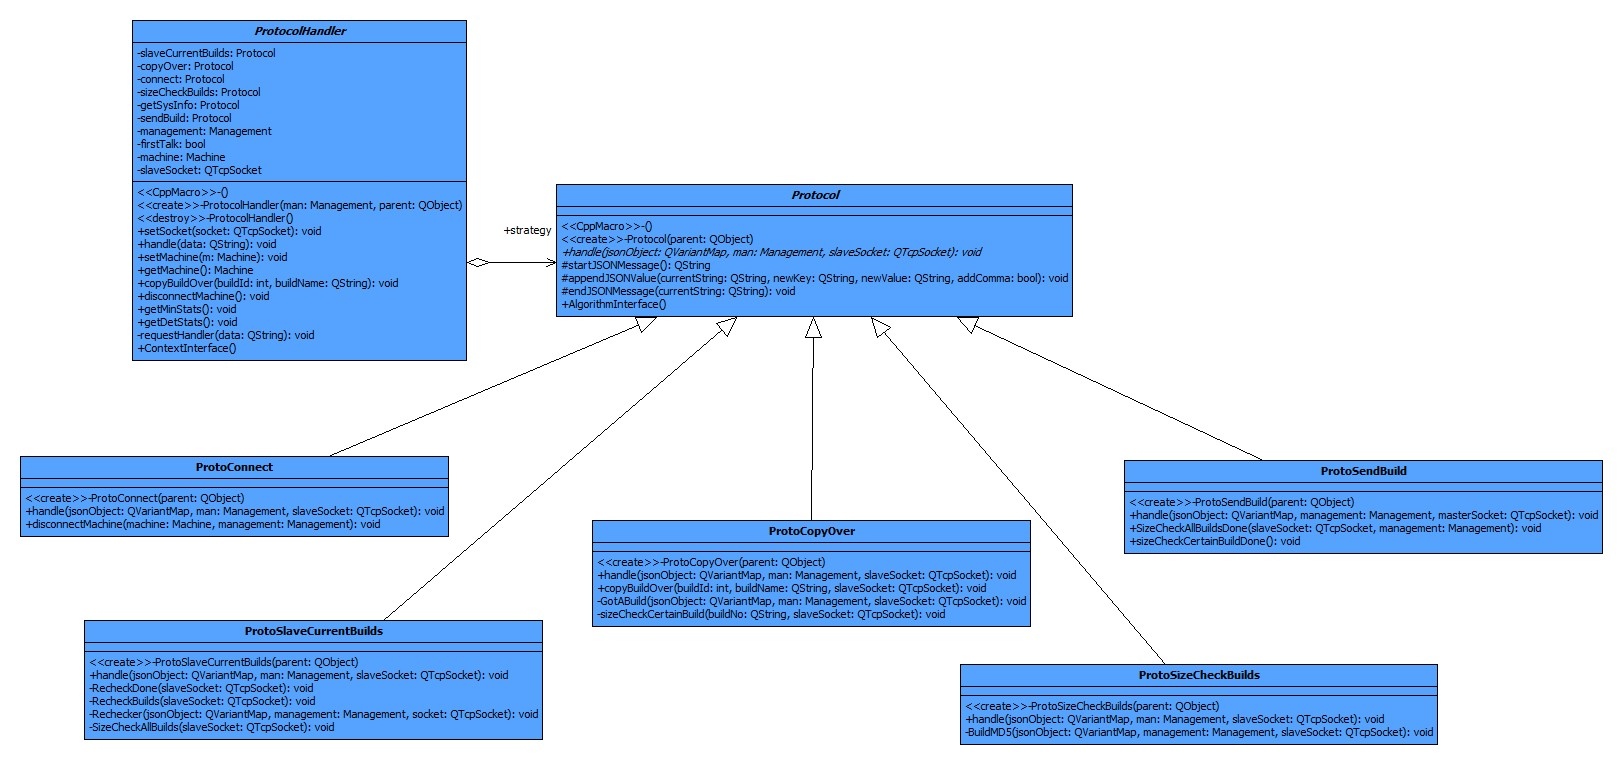
\includegraphics[angle = 90,scale = 0.45]{Protocols.jpg}
\end{center}
\begin{center}
	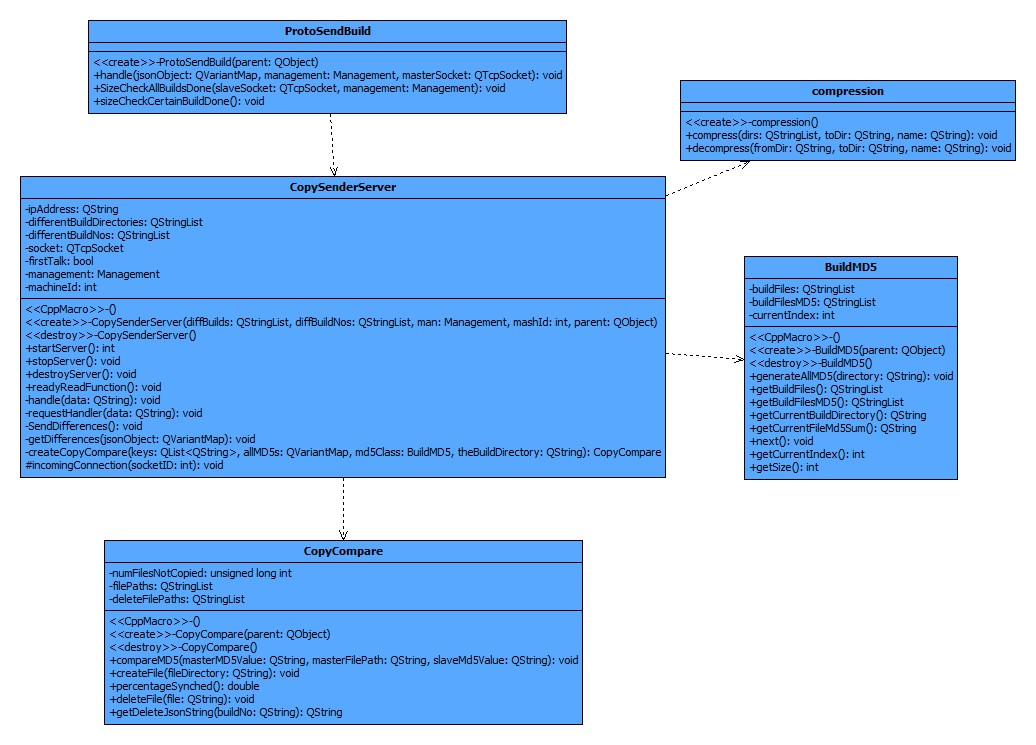
\includegraphics[angle = 90,scale = 0.65]{BuildCopy.jpg}
\end{center}
\begin{center}
	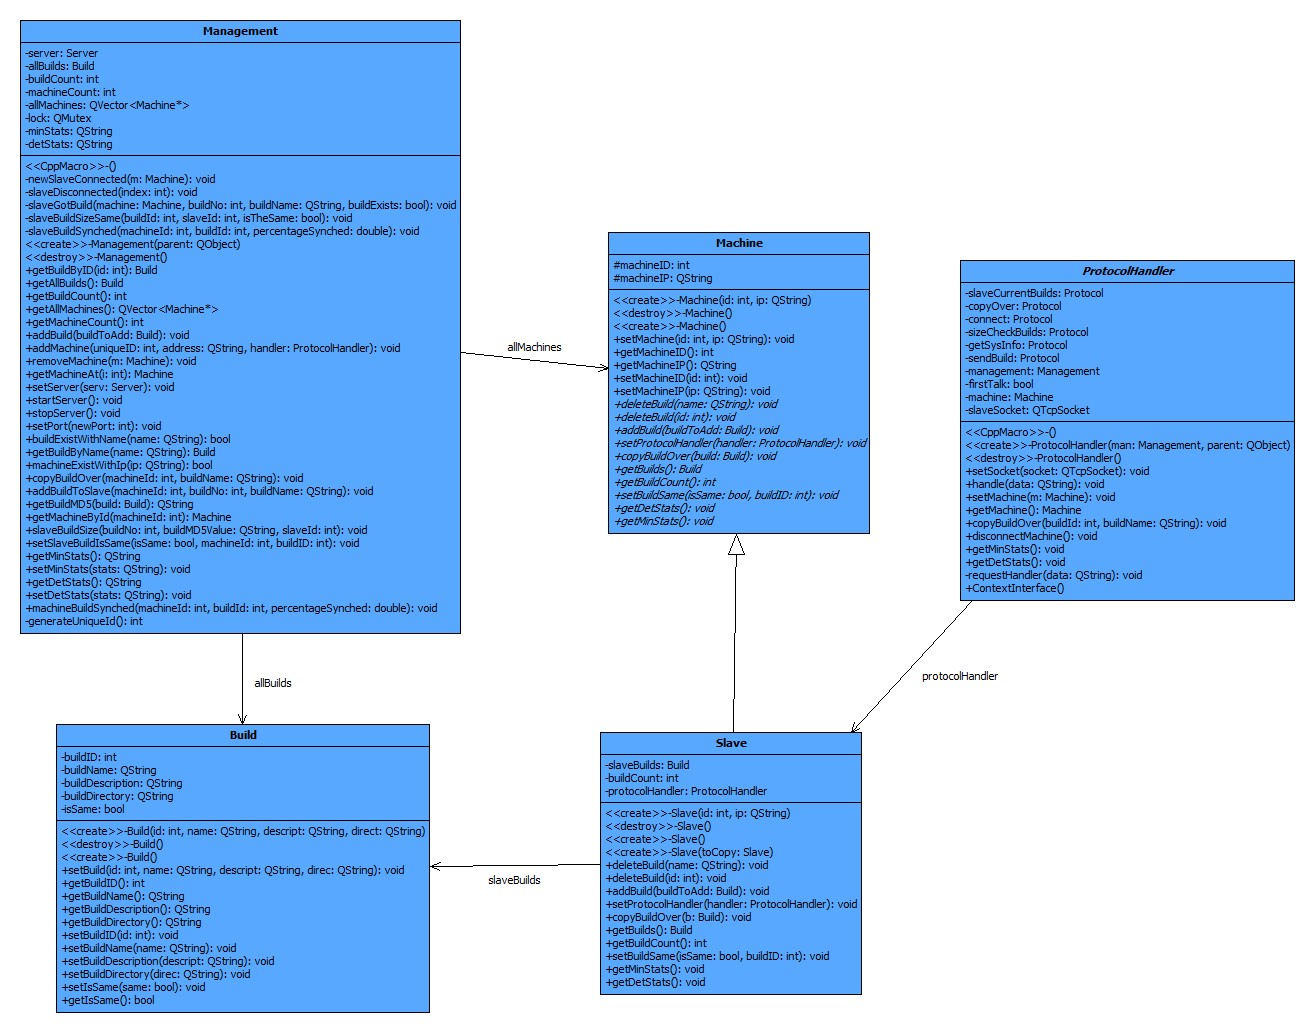
\includegraphics[angle = 90,scale = 0.47]{Slave.jpg}
\end{center}
\newpage
\subsection{AppManClient Class Diagram}
Due to its large size, the class diagram is split into multiple, seperate diagrams. Classes will be repeated to show how they all link.\\
\begin{center}
	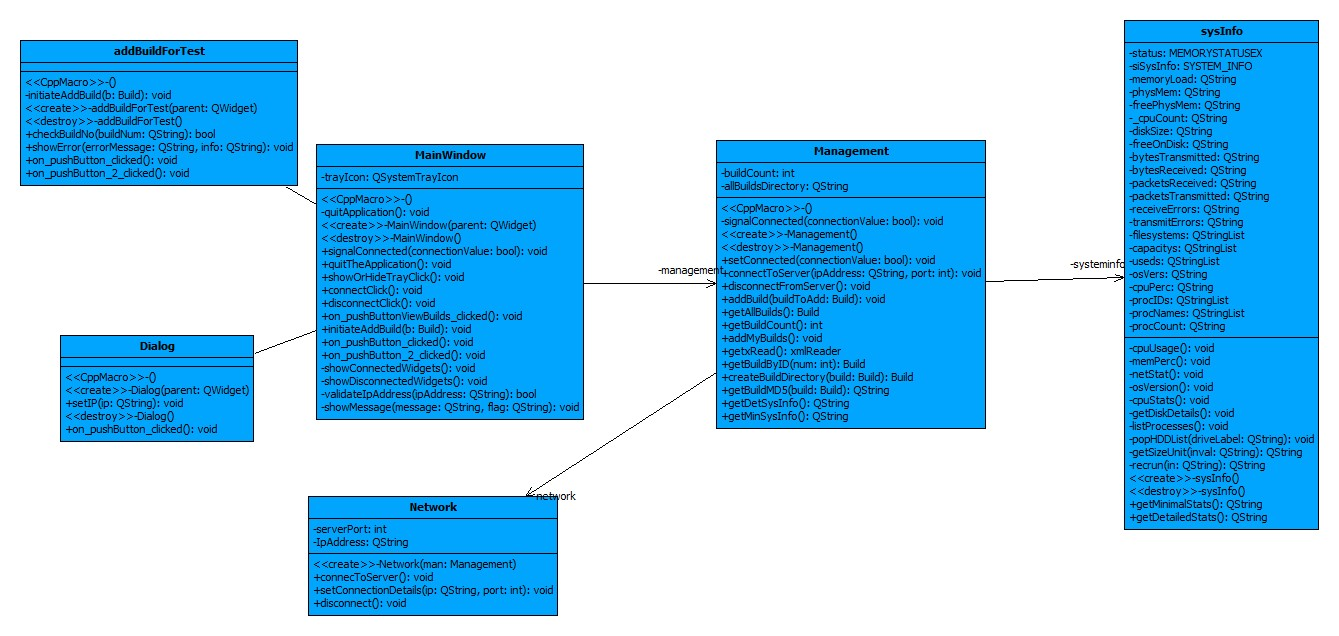
\includegraphics[angle = 90,scale = 0.47]{Part1.jpg}
\end{center}
\begin{center}
	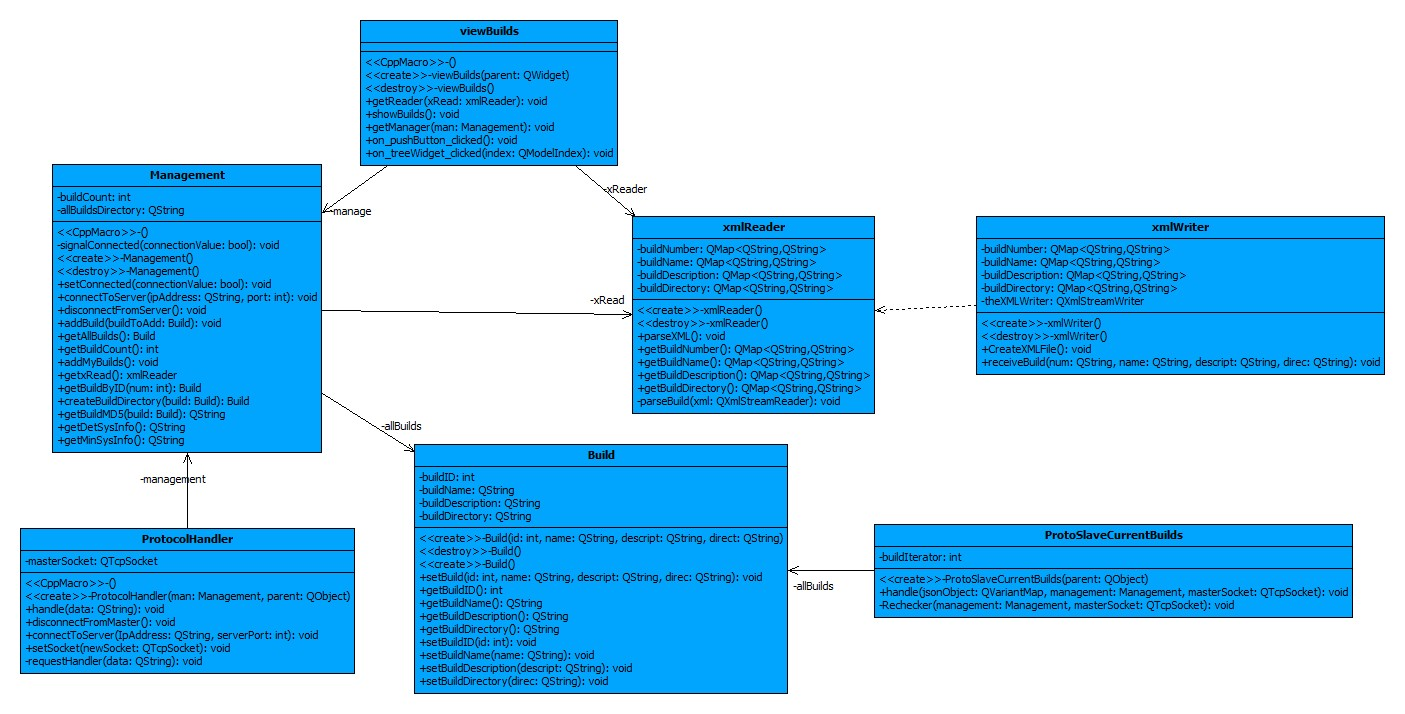
\includegraphics[angle = 90,scale = 0.47]{Part1_1.jpg}
\end{center}
\begin{center}
	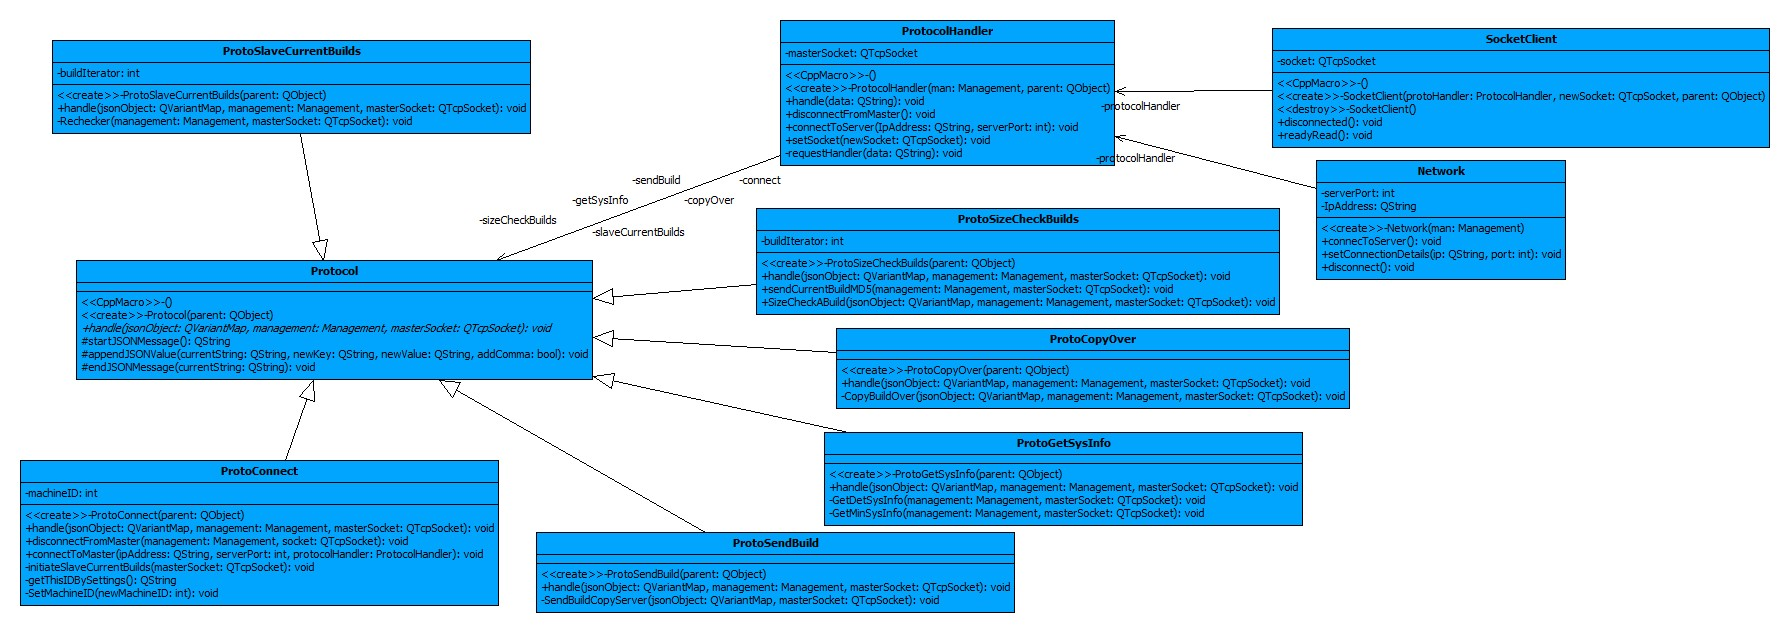
\includegraphics[angle = 90,scale = 0.4]{Part2.jpg}
\end{center}
\begin{center}
	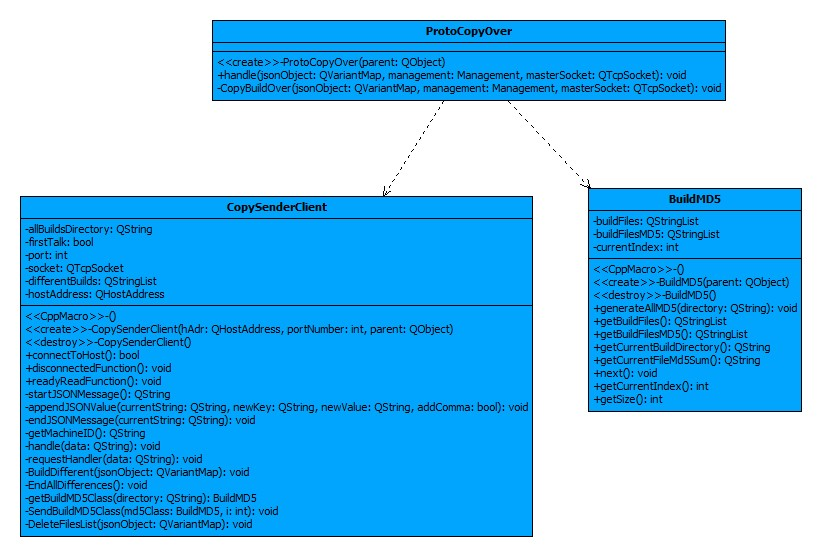
\includegraphics[angle = 90,scale = 0.7]{Part3.jpg}
\end{center}


\newpage
\section{Overall Processes}
This section is for the Activity diagrams based on current progress of AppMan and AppManClient respectively.
\subsection{AppMan}
\begin{center}
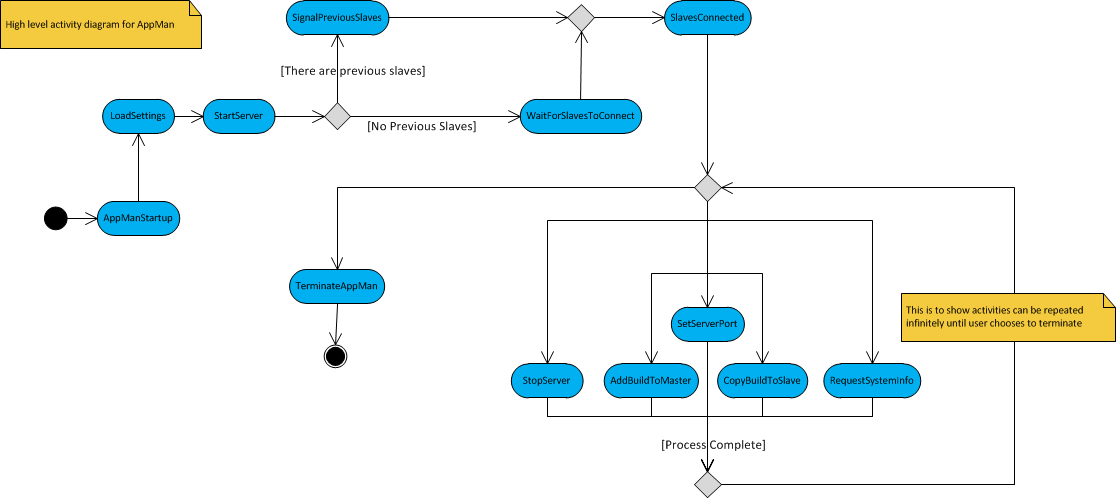
\includegraphics[angle = 90, scale=0.7]{MasterMainActivity.png}
\end{center}
\newpage
\subsection{AppManClient}
\begin{center}
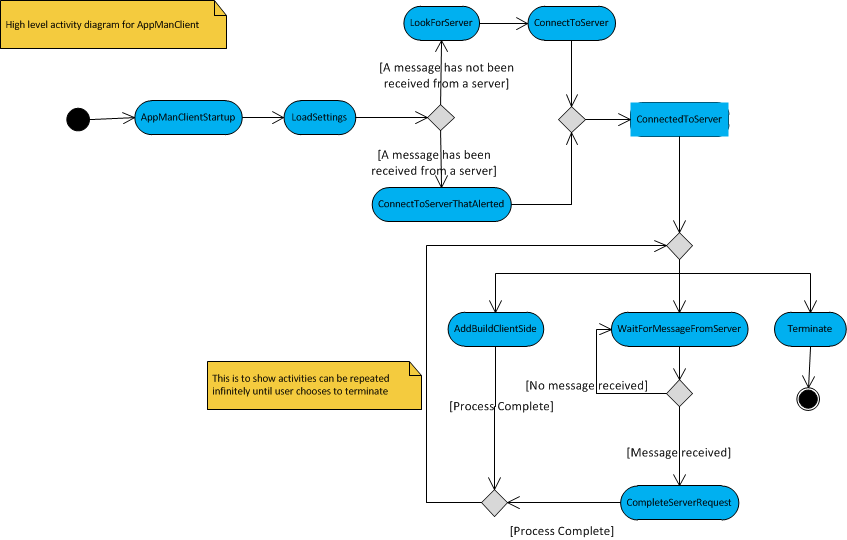
\includegraphics[angle = 90, scale=1]{SlaveMainActivity.png}
\end{center}



\newpage
\section{Communication Protocol}
\subsection{Overview}
The communication between AppMan and AppManClient takes place 
by using JSON objects. The JSON objects are structured such that the 
content of the JSON message govern where the message will be handled. 
The communication protocol inside the application is set in a strategy design pattern
whereby the context is passed on from the protocol handler to the class that will 
handle the data. This strategy design pattern is mirrored on the master and the slave
machine to link each strategy to its partner on the other application(i.e. master to slave).
The concrete strategies are the classes that handle all the data as JSON objects.\\
\textbf{\\}
The JSON for normal communication is in the following format:
\begin{verbatim}
{
	"handler" : "[  The Handler ] ",
	"subHandler" : "[ The SubHandler  ]"
	"data" :  "[ Field values ]"
}
\end{verbatim}
The ProtocolHandler will firstly look at the handler and based on that it will decide to
which concrete strategy it should be passed on. The handler will be a string that contains
the name of the concrete strategy to handle the request. After the handler has been 
identified the data and all other applicable data are passed on to the concrete strategy.\\
\textbf{\\}
After it has arrived at one of the concrete strategies, the function will look at what
the subHandler is. Based on the value of the subHandler, it calls the function labeled
to that subhandler by passing the data on to that subHandler.\\
\textbf{\\}
The data in the JSON object can be a variety of variables ranging from build number
to machine ID. This is set in the JSON object and is retrieved by the handler depending
on when they need to use it.\\
\textbf{\\}

\subsection{Strategies}
The strategy design pattern is easy to adapt and add new classes in order to include
new strategies for other application communications to take place. The current concrete
strategies are:
\begin{itemize}
\item ProtoConnect
\item ProtoSlaveCurrentBuilds
\item ProtoSizeCheckBuilds
\item ProtoCopyOver
\item ProtoSendBuild
\end{itemize}

ProtoConnect: This strategy will be used in the event that a new client tries to connect. If 
the correct protocol is not followed in the event of a connection, the socket will be disconnected.
If the client successfully connects the strategy will create a new machine and allow the user to
interact with that machine. After a machine connected this protocol will invoke the ProtoSlaveCurrentBuilds
which will update what builds are currently on the slave machine.
\\
\textbf{\\}
ProtoSlaveCurrentBuilds: This strategy will be invoked each time the slave machine 
acknowledges a new build that they now have. This can be invoked by the ProtoConnect or
ProtoCopyOver. In the event of the ProtoConnect all the builds that are on the slave machine are
communicated to the master machine. In the event of ProtoCopyOver, only the new build that
has been copied over is communicated.
\\
\textbf{\\}
ProtoSizeCheckBuilds: This strategy is used to find the md5 sum values of the whole 
directory in which the builds are located. The md5 sum values are calculated for the whole
build directory whereby it checks whether the md5 sum values of the master and slave for the
same build are the same. It then updates the interface to show whether the build is the right size. 
This strategy can be invoked by the ProtoCurrentBuilds right after the current builds has been
updated on the master machine, in which case each and every build md5 is generated. In the case
of ProtoCopyOver invoking this strategy, only the new build that is to be copied over will have the md5
generated for it.
\\
\textbf{\\}
ProtoCopyOver: This strategy is used to communicate a new bulid that should be copied over
from the master to the slave machine. The strategy will update on the master only when the
slave machine has confirmed the presence of a new build that should be on it. 
\\
\textbf{\\}
ProtoSendBuild: This strategy will communicate when there needs to be a new build that
must be copied over the network from the master to the slave machine. The master machine will
create another server by which the slave build connects to.
\\
\textbf{\\}
Future expansion will include the following
\begin{itemize}
\item ProtoSimulations
\item ProtoUpdate
\end{itemize}

ProtoSimulations: This protocol will be used to run simulations on the slave machine by running
applications with the application configuration.\\
\textbf{\\}
ProtoUpdate: This is a communication protocol which will be used in order to update build
information or other information on the slave machines.



\newpage
\section{Glossary}
\begin{itemize}
\item{Build - An application build version that could potentially be distributed to slave computers.}
\item{Slave - A computer that will be controlled via a master computer. Application builds will be sent to this computer.}
\item{Master - A computer that will control Slaves across a network.}
\item{Server - A machine waiting on the network for connections from other machines.}
\item{GUI - Graphical User Interface with which a user can control the project.}
\item{Project - This project. The distributed application manager.}
\item{Application - A 3rd party program the client may use during simulations}
\end{itemize}




\end{document}